% !TeX root = main.tex
% !TEX TS-program = pdflatex
\documentclass[stu, babel, american, biblatex, a4paper, draftall]{apa7}
% APA related headers
% https://apastyle.apa.org/style-grammar-guidelines
\usepackage{csquotes}
\addbibresource{lists/prelimitary.bib}
\DeclareLanguageMapping{american}{american-apa}
% ASM related headers (Check APA first)
% https://www.ams.org/publications/authors/AMS-StyleGuide-online.pdf
\usepackage{amsmath, amsfonts, amssymb, amsthm}
\usepackage{mathtools}
\usepackage{thmtools}
% other headers for specific purpose (Check APA and ASM first)
\usepackage{tensor}
\usepackage{braket}
\usepackage{hyperref}
\usepackage[capitalise, sort&compress, noabbrev]{cleveref}
\iffalse % memory exceeded, import .pdf instead.
\iffalse % standalone subpreambles invoke errors, manually import instead.
\usepackage[subpreambles=true]{standalone}
\else
\usepackage{standalone}

\usepackage{pgf-umlcd}
\usepackage{pgfplots}
\pgfplotsset{compat=newest}

% \usetikzlibrary{external}
% \tikzexternalize
\fi
\usepackage{import}
\else
\graphicspath{{./figures/}}
\fi

\allowdisplaybreaks
\crefname{paragraph}{paragraph}{paragraphs}
\Crefname{paragraph}{Paragraph}{Paragraphs}
\crefname{subparagraph}{subparagraph}{subparagraphs}
\Crefname{subparagraph}{Subparagraph}{Subparagraphs}


\title{Prove of Constant Radius Model}
\shorttitle{30MA19-02}
\leftheader{Bhunambhon, Nonprasart, Maysamat}  % Author's last names
\authorsnames{Sivakorn Bhunambhon, Hanchai Nonprasart, Sakepisit Maysamat}
\authorsaffiliations{Mahidol Wittayanusorn School}
\course{SCI 30196: Science Project 1}
\professor{Amornsri Amornvatcharapong, Teerapong Suksumran}
\duedate{\today} % Last edit day when the draft watermark is removed.
\abstract{This is the first generation of the model. It's a draft. Who would even care to read the abstract when it's not done anyways?}
\keywords{None 1, None 2, None 3}

%!TEX root = main.tex

% "well-known" notations
\newcommand{\real}{\mathbb{R}}
\newcommand{\nat}{\mathbb{N}}
\newcommand{\inner}[2]{\left\langle{#1},{#2}\right\rangle}
\DeclareMathOperator{\sign}{sgn}
\DeclareMathOperator{\abs}{abs}

% Notation used without definition
\newcommand{\defeq}{\vcentcolon=} % To declare equation as define so there's no need to prove

% notation which may required some prelimitaries or definition
\DeclareMathOperator{\ortho}{O}
\DeclareMathOperator{\genlin}{GL}
\DeclareMathOperator{\euclid}{Euc}
\newcommand{\range}[2]{\set{#1..#2}}

% placeholder commands - Use to find it easier with Ctrl+F
\newcommand{\skipped}{The proof is left as an exercise to the other author.}  % pending proof - JUST DO IT ALREADY
\newcommand{\citenone}{*Not Cited*}  % pending citation - JUST DO IT ALREADY
\newcommand{\proto}[1]{#1...}  % pending operation
\newcommand{\proofof}[1]{Proof of \cref{#1}} % Proof name
\newcommand{\toshowthat}[1]{To show that #1} % Subproof name
\newenvironment{subproof}[1]{%
    \renewcommand{\qedsymbol}{}
    \begin{proof}[To show that #1]$ $\par\nobreak\ignorespaces
        }{%
    \end{proof}
}

% defined notations
\newcommand{\elements}{\mathbb{M}}
\newcommand{\groupoperation}[1]{\otimes_{#1}}
\newcommand{\points}[1]{\mathbb{P}_{#1}}
\newcommand{\transformations}[1]{\mathbb{T}_{#1}}
\newcommand{\group}[1]{\mathbb{G}_{#1}}
\newcommand{\subgroup}[1]{\mathbb{H}_{#1}}
\newcommand{\charts}[1]{\varphi_{#1}}
\newcommand{\innerprod}[1]{g_{#1}}
\declaretheorem[
    name=Definition,
    style=definition,
    refname={definition,definitions},
    Refname={Definition,Definitions},
]{definition}
\declaretheorem[
    name=Example,
    parent=definition,
    style=definition,
    refname={example,examples},
    Refname={Example,Examples},
]{example}  % Use to clearify the definition
\declaretheorem[
    name=Theorem,
    style=plain,
    refname={theorem,theorems},
    Refname={Theorem,Theorems},
]{theorem}
\declaretheorem[
    name=Lemma,
    style=plain,
    refname={lemma,lemmas},
    Refname={Lemma,Lemmas},
]{lemma}
\declaretheorem[
    name=Corollary,
    style=plain,
    refname={corollary,corollaries},
    Refname={Corollary,Corollaries},
]{corollary}
\declaretheorem[
    name=Conjecture,
    style=plain,
    refname={conjecture,conjectures},
    Refname={Conjecture,Conjectures},
]{conjecture}


\newcounter{Counter}

\theoremstyle{definition}
\newtheorem{ModelGroupElement}{Definition}[Counter]
\newtheorem{ModelMetric}[ModelGroupElement]{Definition}

\theoremstyle{plain}
\newtheorem{ModelGroupAssertion}{Assertion}[Counter]
\newtheorem{ModelCurvatureAssertion}[ModelGroupAssertion]{Assertion}

\begin{document}
\maketitle
\tableofcontents

\section{Rewrite note}
This proof will be organized using the following guideline
\begin{APAenumerate}
    \item reviewing existing definitions and theorem
    \item proving certain property of existing mathematical objects
    \item defining the conditions of the model
    \item formulating of the model
    \item parametrizing the model
    \item asserting defined property of the model
\end{APAenumerate}
It turned out that figures will crash overleaf, if you want to view such file, please compile them seperately.
To merge the file, it is needed to either pay the subscription or download and run it on your computer.

\section{Prelimitary}
All citation must goes here,
Authors must copy statement they wanted to cite according to the AMS guideline,
Any theorem lemma definitions and others must be in theorem environment if possible (see amsthm user-guide for more details),
Authors then refer to the statement using {\textbackslash}label\{\} and {\textbackslash}cref\{\}.
\subsection{Uncited prelimitary}
\begin{equation}\label{MatrixMultiplication}
    \tensor{C}{}=\tensor{A}{}\tensor{B}{}
    \iff
    \tensor{C}{^i_j}=\sum_k\tensor{A}{^i_k}\tensor{B}{^k_j}
\end{equation}
\begin{definition}\label{KleinGeometry}
    KleinGeometry
\end{definition}
\begin{example}\label{KleinGeometryExample}
    KleinGeometryExamples (I)
\end{example}

\section{Objective}
\stepcounter{Counter}
\paragraph{Objective}\label{Objective}
The objective is to construct
\begin{APAenumerate}
    \item a set $M$
    \item an $n$-dimensional $C^\infty$ differential structure on set $M$ with chart $\varphi\in M\to\real^n$ (which give it a manifold structure)
    \item an algebralic structure (group) on $M$ with operation $\otimes$ (since identity, invertibility, and associativity apply to distance-preserving (curvature-preserving) transformations in the geometry)
    \item an metric space on $M$ with metric $d\in M\times M\to\real$
\end{APAenumerate}
(to be determined)
such that
\begin{APAitemize}
    \item all of its two-dimensional linear subspaces have sectional curvature of $\kappa$
    \item $d\left(\varphi^{-1}\left(x\right), \varphi^{-1}\left(y\right)\right)$ is infinitely differentiable by $\kappa$ for all $x$ and $y$ in $\real^n$
\end{APAitemize}
given a natural number $n$ and a real number $\kappa$.

\subparagraph{Algorithm}\label{ModelAbstractClass}
(see \cref{ModelClassDiagram})

\begin{definition}\label{SetOfPoints}
    \textit{Set of points} $\points{M}$ is defined as set of equivalence classes of elements of $M$ with the relation $r$,
    where $r\defeq\Set{\left(x,y\right)\in M\times M | d(x,y)=0}$
    (Generally speaking, distance between those two elements are zero).
\end{definition}
\begin{definition}\label{SetOfTransformations}
    \textit{Set of transformations} $\transformations{M}$ is defined as
    $\transformations{M}\defeq\Set{f\in M \to M | \exists y \in M, f\left(x\right) = y \otimes x}$.
\end{definition}
\begin{definition}\label{ModelGroup}
    \textit{Principal group} and \textit{subgroup} of the model is defined as
    \begin{APAitemize}
        \item Let $\group{M}$ be a group on set $M$ together with binary operation $\otimes$.
        \item Let $\subgroup{M}$ be a group on set $P\in\points{M}$ together with binary operation $\otimes$.
    \end{APAitemize}
    respectively.
\end{definition}
\begin{conjecture}\label{GeometricGroupStructure}
    If parameters $\left(\kappa,n\right)$ is associated with Klein geometry $\left(G,H\right)$
    then $\group{M}\cong G$ and $\subgroup{M}\cong H$.

    From \cref{KleinGeometryExample},
    \begin{APAitemize}
        \item For $\kappa>0$, $\group{M}\cong\ortho\left(n+1\right)$ and $\subgroup{M}\cong\ortho\left(n\right)$.
        \item For $\kappa=0$, $\group{M}\cong\euclid\left(n\right)$ and $\subgroup{M}\cong\ortho\left(n\right)$.
        \item For $\kappa<0$, $\group{M}\cong\ortho^{+}\left(1,n\right)$ and $\subgroup{M}\cong\ortho\left(n\right)$.
    \end{APAitemize}
\end{conjecture}
\section{Model Foundation}
\proto{Construction of the set $M$}
\subsection{Trigonometry}
\begin{definition}\label{Trigonometry}
    \textit{Generalized trigonometric functions} $f_k:\mathbb{R}\to\mathbb{R}$ are defined as
    \begin{align*}
        f_k\left(\theta\right) & \defeq
        \begin{cases}
            g\left(k\theta\right) & \text{if $k\geq0$,} \\
            h\left(k\theta\right) & \text{otherwise,}   \\
        \end{cases}
    \end{align*}
    where $g$ (resp. $h$) are the associated trigonometric (resp. hyperbolic) function.
\end{definition}
\begin{example}\label{TrigonometrySine}
    \textit{Generalized sine function} (see \cref{TrigonometrySinePlotted}) is defined as
    \begin{align*}
        \sin_k{\theta} & \defeq
        \begin{cases}
            \sin\left(k\theta\right)  & \text{if $k\geq0$,} \\
            \sinh\left(k\theta\right) & \text{otherwise.}   \\
        \end{cases}
    \end{align*}
\end{example}
\begin{example}\label{TrigonometryCosine}
    \textit{Generalized cosine function} (see \cref{TrigonometryCosinePlotted}) is defined as
    \begin{align*}
        \cos_k{\theta} & \defeq
        \begin{cases}
            \cos\left(k\theta\right)  & \text{if $k\geq0$,} \\
            \cosh\left(k\theta\right) & \text{otherwise.}   \\
        \end{cases}
    \end{align*}
\end{example}
\begin{example}\label{TrigonometryTangent}
    \textit{Generalized tangent function} (see \cref{TrigonometryTangentPlotted}) is defined as
    \begin{align*}
        \tan_k{\theta} & \defeq
        \begin{cases}
            \tan\left(k\theta\right)  & \text{if $k\geq0$,} \\
            \tanh\left(k\theta\right) & \text{otherwise.}   \\
        \end{cases}
    \end{align*}
\end{example}
\begin{corollary}\label{TrigonometryContinuity}
    Generalized sine and cosine function are infinitely differentiable.
\end{corollary}
\begin{proof}[\proofof{TrigonometryContinuity}]
    % Since $\sin$, $\cos$, $\sinh$, and $\cosh$ are infinitely differentiable,
    % $\sin_k$ and $\cos_k$ are infinitely differentiable by $\theta$
    % and $\sin_k$ and $\cos_k$ are infinitely differentiable by $k$ at $k\ne0$.

    % \begin{align*}
    %     \frac{d}{dk}\sin_k^{\prime}\theta\left(0\right)
    %      & = \lim_{h\to0}\frac{\sin_{h}\theta-\sin_{-h}\theta}{2h}                          \\
    %      & = \lim_{h\to0}\frac{\sin{\left(h\right)\theta}-\sinh{\left(-h\right)\theta}}{2h} \\
    %      & = \lim_{h\to0}\frac{\left(h\right)\theta-\left(-h\right)\theta}{2h}              \\
    %      & = \lim_{h\to0}\theta                                                             \\
    %      & = \theta
    % \end{align*}

    % Since $\sin^{\prime}\theta=\cos\theta$ and $\sinh^{\prime}\theta=\cosh\theta$,
    % \begin{align*}
    %     \sin_k^{\prime}\theta
    %      & =
    %     \begin{cases}
    %         \theta\cos{k\theta}  & \text{if $k>0$,} \\
    %         \theta               & \text{if $k=0$,} \\
    %         \theta\cosh{k\theta} & \text{if $k<0$.} \\
    %     \end{cases} \\
    %      & = \theta\cos_k{\theta}
    % \end{align*}

    % Similarly, $\cos_k^{\prime}=-\sign{\left(k\right)}\theta\sin_k{\theta}$.

    \skipped

    By using mathematical induction, it can be proved that
    \begin{align*}
        \sin_k^{\left(4n\right)}\theta   & = \theta^{4n}\sin_k{\theta}                         \\
        \cos_k^{\left(4n\right)}\theta   & = \theta^{4n}\cos_k{\theta}                         \\
        \sin_k^{\left(4n+1\right)}\theta & = \theta^{4n+1}\cos_k{\theta}                       \\
        \cos_k^{\left(4n+1\right)}\theta & = -\sign{\left(k\right)}\theta^{4n+1}\sin_k{\theta} \\
        \sin_k^{\left(4n+2\right)}\theta & = -\sign{\left(k\right)}\theta^{4n+2}\sin_k{\theta} \\
        \cos_k^{\left(4n+2\right)}\theta & = -\sign{\left(k\right)}\theta^{4n+2}\cos_k{\theta} \\
        \sin_k^{\left(4n+3\right)}\theta & = -\sign{\left(k\right)}\theta^{4n+3}\cos_k{\theta} \\
        \cos_k^{\left(4n+3\right)}\theta & = \theta^{4n+3}\sin_k{\theta}
    \end{align*}
    Hence, generalized sine and cosine function can be infinitely differentiable.
\end{proof}
\begin{theorem}[Pythagorean's identity equivalence]\label{TrigonometryPythagorean}
    \begin{align*}
        \cos_k^2{\theta} & +\sign{k}\sin_k^2{\theta} & = 1                \\
        1                & +\sign{k}\tan_k^2{\theta} & = \sec_k^2{\theta} \\
        \cot_k^2{\theta} & +\sign{k}                 & = \csc_k^2{\theta}
    \end{align*}
\end{theorem}
\begin{proof}[\proofof{TrigonometryPythagorean}]
    \skipped

    Proof by exhaustion. (Proof by cases.)
\end{proof}
\subsection{Matrices}
\begin{definition}\label{RotationMatrix}
    \textit{Generalized rotation matrix} is defined as
    \begin{align*}
        R_k\left(\theta\right) & \defeq
        \begin{bmatrix}
            \cos_k{\theta}  & \sin_k{\theta} \\
            -\sin_k{\theta} & \cos_k{\theta} \\
        \end{bmatrix}\text{,}
    \end{align*}
    where $\theta\in\real$.
\end{definition}
\begin{definition}\label{PositionMatrix}
    \textit{Position matrix} is defined recursively as
    \begin{align*}
        P_{k,n}\left(\left\{\tensor{\theta}{^1},\dots,\tensor{\theta}{^n}\right\}\right) & \defeq
        \begin{bmatrix}
            P_{k,n-1}\left(\left\{\tensor{\theta}{^1},\dots,\tensor{\theta}{^{n-1}}\right\}\right) & 0 \\
            0                                                                                      & 1 \\
        \end{bmatrix}
        T_\pi
        \begin{bmatrix}
            R_k\left(\tensor{\theta}{^n}\right) & 0 \\
            0                                   & I \\
        \end{bmatrix}
        T_\pi \text{,}                                                                                        \\
        P_{k,0}                                                                          & \defeq I_1\text{,}
    \end{align*}
    where $\pi=\begin{pmatrix}
            1 & 2   & 3 & \dots & n & n+1 \\
            1 & n+1 & 3 & \dots & n & 2   \\
        \end{pmatrix}$
    and $\theta=\left\{\tensor{\theta}{^i}\right\}\in\real^n  \text{for } i\in\range{1}{n}$.
\end{definition}
\begin{definition}\label{OrientationMatrix}
    \textit{Orientation matrix} is defined as
    \begin{align*}
        O^\pm_n\left(\phi_{n-1},\phi_{n-2},\dots,\phi_1\right) & \defeq
        \begin{bmatrix}
            1 & 0                                                             \\
            0 & X^\pm_{+1,n-1}\left(\phi_{n-1},\phi_{n-2},\dots,\phi_1\right) \\
        \end{bmatrix}\text{,}                                              \\
        O^\pm_0                                                & \defeq \pm I_1\text{,}
    \end{align*}
    where $\phi_m\in\real^m \text{for } m\in\range{1}{n-1}$.
\end{definition}
\begin{definition}\label{PointMatrix}
    \textit{Point matrix} is defined as
    \begin{align*}
        X^\pm_{k,n}\left(\theta,\phi_{n-1},\phi_{n-2},\dots,\phi_1\right) & \defeq
        P_{k,n}\left(\theta\right)
        O^\pm_n\left(\phi_{n-1},\phi_{n-2},\dots,\phi_1\right)\text{,}
    \end{align*}
    where $\theta\in\real^n$ and $\phi_m\in\real^m \text{for } m\in\range{1}{n-1}$.
\end{definition}
\subsection{Group structure}
Proof of validity of $\group{M}$ and $\subgroup{M}$ (validity of $\otimes$, proof of the matrices to be $\subgroup{M}$ will later be discussed)...
\begin{lemma}\label{OrientationGroup}
    Orientation matrix with multiplication
    is isomorphic to orthogonal group.
\end{lemma}
\begin{proof}[\proofof{OrientationGroup}]
    Let
    \begin{APAitemize}
        \item the group of orientation matrix $O^{\pm}_{n}$ with multiplication is $\left(P\left(n\right),\cdot\right)$,
        \item the group of point matrix $X^{\pm}_{+1,n-1}$ at $k=+1$ with multiplication is $\left(M\left(n\right),\cdot\right)$.
    \end{APAitemize}

    To shows that $P\left(n\right)\cong M\left(n-1\right)$.
    Consider the mapping
    \begin{align*}
        f      & : X^{\pm}_{+1,n-1}\left(\phi,\dots\right) \mapsto O^{\pm}_{n}\left(\phi,\dots\right) & \in M\left(n-1\right) \to P\left(n\right) \text{,} \\
        f^{-1} & : O^{\pm}_{n}\left(\phi,\dots\right) \mapsto X^{\pm}_{+1,n-1}\left(\phi,\dots\right) & \in P\left(n\right) \to M\left(n-1\right) \text{,}
    \end{align*}
    which by \cref{OrientationMatrix} is equivalent to
    \begin{equation} \label{PointToOrientationIsomorphism}
        f : X \mapsto \begin{bmatrix}
            1 & 0 \\
            0 & X \\
        \end{bmatrix}
        \text{.}
    \end{equation}

    For any point matrices $X_1, X_2 \in M\left(n-1\right)$, it can be shown that
    \begin{align}
        f\left(X_1\right)\cdot f\left(X_2\right)
                                                 & =\begin{bmatrix}
            1 & 0   \\
            0 & X_1 \\
        \end{bmatrix}\cdot\begin{bmatrix}
            1 & 0   \\
            0 & X_2 \\
        \end{bmatrix}                         &  & \text{(substitute \cref{PointToOrientationIsomorphism})} \nonumber \\
                                                 & =\begin{bmatrix}
            1 & 0            \\
            0 & X_1\cdot X_2 \\
        \end{bmatrix}                                                        &  & \text{(simplify)} \nonumber                                        \\
        f\left(X_1\right)\cdot f\left(X_2\right) & = f\left(X_1\cdot X_2\right)\text{.} \label{PointToOrientationIsomorphismProperty}
    \end{align}
    Therefore, $P\left(n\right)\cong M\left(n-1\right)$.

    Hence, it is sufficient to shows that $M\left(n-1\right)\cong O\left(n\right)$.

    To show that the isomorphism is the identity mapping
    (to shows that $M\left(n-1\right)=O\left(n\right)$)
    is sufficient to shows that
    \begin{APAenumerate}
        \item Every points matrices $X \in M\left(n-1\right)$ is an element of orthogonal group $\ortho\left(n\right)$.
        \item Every orthogonal matrices $A \in \ortho\left(n\right)$ is an point matrix in $M\left(n-1\right)$.
    \end{APAenumerate}

    To show that
    \begin{align*}
        \forall n\in\nat, \forall X\in M\left(n-1\right),
             & X\in \ortho\left(n\right)                                  \\
        \iff & X\in \set{A\in\genlin\left(n\right)\mid A A^T = A^T A = I} \\
        \iff & X\in\genlin\left(n\right) \wedge A A^T = A^T A = I\text{.}
    \end{align*}
    \begin{proof}
        It is obvious that $X$ is an $n$-by-$n$ square matrix.

        And if $X$ is orthogonal ($X X^T = X^T X = I$),
        then there exist an $n$-by-$n$ square matrix $Y = X^T$ such that $X Y = Y X = T$ ($X$ is invertible).

        Hence, it is sufficient to shows that $X$ is orthogonal.

        To show that $X$ is orthogonal.

        \skipped

        Use closed property of orthogonal group.

        It can be proved that position matrix with such parameter (or its factor) is orthogonal.

        It can also be prove inductively that orthogonal matrix is orthogonal by using its block form and base case of point matrix.
    \end{proof}
    To show that $\forall n\in\nat, \forall A\in \ortho\left(n-1\right), \exists X\in M\left(n-1\right), A=X$.
    \begin{proof}
        \skipped

        No idea on how to prove yet.
    \end{proof}
\end{proof}
\begin{lemma}\label{PointGroup}
    Point matrix with multiplication
    is isomorphic to principal group of the associated Klein geometry.
\end{lemma}
\begin{proof}[\proofof{PointGroup}]
    \skipped

    Spherical case is proved successfully with \cref{OrientationGroup}.

    Euclidean case should use limits and first degree taylor series.

    hyperbolic case is similar to \cref{OrientationGroup} such that it use closed property.
\end{proof}
\begin{lemma}\label{PositionGroup}
    Position matrix is isomorphic to quotient group of the associated Klein geometry.
\end{lemma}
\begin{proof}[\proofof{PositionGroup}]
    \skipped

    It can be seen that $Q\cong M/P \iff M \cong Q \ltimes P$,
    point matrix is isomorphic to the principal group,
    orientation matrix is isomorphic to the subgroup,
    and point matrix is product of position and orientation matrix.

    They may be useful for proving that is not yet to be known.

    Another way is to seek for general form of the matrix element of the group of the Klein geometry.
\end{proof}
\section{Model Parametrization}
\proto{Construction of the charts $\varphi$}
\begin{definition}\label{PositionParameter}
    For point matrix $\tensor{X^\pm_{k,n}\left(\theta,\phi_1,\phi_2,\dots,\phi_n\right)}{}$,
    $n$-dimensional vector $\tensor{\theta}{}$
    is defined as \textit{position parameter}.
\end{definition}
\begin{definition}\label{PositionVector}
    For point matrix $\tensor{X}{}$,
    $\left(n+1\right)$-dimensional column vector $\tensor{p}{}\defeq \tensor{X}{}\cdot\tensor{e}{^1}=\tensor{X}{_1}$
    is defined as \textit{position vector}.
\end{definition}
\proto{This will provide a hint on why the matrices are $\subgroup{M}$...}
\begin{lemma}\label{PositionVectorMatrix}
    For point matrix $X=PO$
    where $P$ and $O$ are position and orientation matrix respectively,
    $\tensor{p}{}=\tensor{X}{_1}=\tensor{P}{_1}$.
\end{lemma}
\begin{proof}[\proofof{PositionMatrix}]
    From \cref{OrientationMatrix}, it is obvious that
    \begin{equation}\label{OrientationColumn}
        \tensor{O}{^i_1} =
        \begin{cases}
            1 & \text{if $i=1$,}  \\
            1 & \text{otherwise.} \\
        \end{cases}
    \end{equation}
    \begin{align*}
        \tensor{p}{^i}
         & = \tensor{X}{^i_1}                         &  & \text{From \cref{PositionVector}}       \\
         & = \sum_j{\tensor{P}{^i_j}\tensor{O}{^j_1}} &  & \text{From \cref{MatrixMultiplication}} \\
         & = \tensor{P}{^i_1}                         &  & \text{From \cref{OrientationColumn}}    \\
        \tensor{p}{}
         & = \tensor{X}{_1}                                                                        \\
         & = \tensor{P}{_1}                           &  & \qedhere
    \end{align*}
\end{proof}
\begin{lemma}\label{PositionVectorValue}
    Given position parameter $\tensor{\theta}{}$, position vector can be evaluated as the following.
    \begin{align*}
        \tensor{p}{} & =
        \begin{pmatrix}
            \prod_{j\in\Set{1..n}}{\cos_k{\tensor{\theta}{^j}}}                                \\
            \sin_k{\tensor{\theta}{^{i-1}}}\prod_{j\in\Set{i..n}}{\cos_k{\tensor{\theta}{^j}}} \\
            \sin_k{{\tensor{\theta}{^n}}}                                                      \\
        \end{pmatrix}\text{.}
    \end{align*}
\end{lemma}
\begin{proof}[\proofof{PositionVectorValue}]
    \skipped

    Use \cref{PositionVectorMatrix} and recursively compute the vector.
\end{proof}
\begin{lemma}\label{PositionParameterValue}
    Given position vector $\tensor{p}{}$, position parameter can be calculated as the following.
    \begin{align*}
        \tensor{\theta}{} & =
        \begin{pmatrix}
            \arcsin_k{\frac{\tensor{p}{^{i+1}}}{\prod_{j\in\Set{i+1..n}}{\cos_k{\tensor{\theta}{^j}}}}} \\
            \arcsin_k{\tensor{p}{^{n+1}}}                                                               \\
        \end{pmatrix}\text{.}
    \end{align*}
\end{lemma}
\begin{proof}[\proofof{PositionParameterValue}]
    \skipped

    Use \cref{PositionVectorValue} to compute the inverse mapping.
\end{proof}
\proto{Trying to explain how domain of the chart can be seperated in such a way that
there is a bijective mapping between $\tensor{p}{}$ and $\tensor{\theta}{}$}
\paragraph{Coordinate Singularity}
    It can be seen that at $\cos_k{\tensor{\theta}{^j}}=0$,
    $\tensor{\theta}{^i}$ is undefined for $i<j$.
    Such case only occur in spherical geometry at $\tensor{\theta}{^j}=\left(2m\pm\frac{1}{2}\right)\frac{\pi}{k}$,
    which is the pole where coordinate lose its degree of freedom (i.e. gimbal's lock)
    and technically is the boundary of the unique points of single-elliptic geometry.
\paragraph{Parameter Signature}
    In case of $k>0$,
    to assure that the mapping between $\tensor{p}{}$ and $\tensor{\theta}{}$,
    all parameter $\tensor{\theta}{^i}$ is bound to range of $\left(-\frac{1}{2}\frac{\pi}{k},+\frac{1}{2}\frac{\pi}{k}\right)$ for $i\ne1$.
    But given the signature of $\prod_{j\in\Set{1..n}}{\cos_k{\tensor{\theta}{^j}}}$
    and the fact that $\cos_k{\tensor{\theta}{^j}}>0$
    when $k\leq 0$ or $\tensor{\theta}{^j}\in\left(\left(2m-\frac{1}{2}\right)\frac{\pi}{k},\left(2m+\frac{1}{2}\right)\frac{\pi}{k}\right)$,
    one position parameter $\tensor{\theta}{^1}$ can be extended to range of $\left(-1\frac{\pi}{k},+1\frac{\pi}{k}\right)$.
\subsection{Coordinate Mapping}
\proto{Proof of validity of $\phi$}
\begin{corollary}\label{PositionEquivalence}
    Position parameter, position vector, and position matrix
    are equivalence in such ways that
    provided any of them, the others can be calculated.
\end{corollary}
\section{Geometric properties}
\proto{Construction of the metric $d$}
\subsection{Embedding}
\begin{definition}\label{ScaledPositionVector}
    \textit{Scaled position vector} is defined as $\tensor{x}{} = \frac{\tensor{p}{}}{k}$.
\end{definition}
\begin{definition}\label{Embedding}
    Let $M=\left(P,g\right)$ be a $n$-dimension Riemannian manifold
    on position parameter space with such metric that
    the map $\phi:P\to P^{\prime}$
    from position parameter space $P\subset\mathbb{R}^{n}$
    to scaled position vector space $P^{\prime}\subset\mathbb{R}^{n+1}$
    is an isometric embedding to $\left(n+1\right)$-Euclidean manifold.
\end{definition}
\begin{lemma}\label{MetricTensor}
    The metric tensor of $M$ is
    \begin{align*}
        \tensor{g}{_i_j} & =
        \begin{cases}
            \prod_{a>i}{\cos_k^2{\tensor{\theta}{^a}}} & \text{if $i=j$}  \\
            0                                          & \text{otherwise} \\
        \end{cases}
    \end{align*}
\end{lemma}
\begin{proof}[\proofof{MetricTensor}]
    \skipped
\end{proof}
\subsection{Locus of scaled position vector}
\stepcounter{Counter}
\begin{lemma}\label{SphericalLocus}
    For $k>0$, locus of $\phi$ is a $\left(n+1\right)$-sphere of radius $k^{-1}$.
\end{lemma}
\begin{proof}[\proofof{SphericalLocus}]
    \skipped

    Use \cref{TrigonometryPythagorean} and et cetera.
\end{proof}
\begin{lemma}\label{HyperbolicLocus}
    For $k<0$, locus of $\phi$ is a forward sheet of a two-sheeted $\left(n+1\right)$-hyperboloid of radius $k^{-1}$.
\end{lemma}
\begin{proof}[\proofof{HyperbolicLocus}]
    \skipped

    Use \cref{TrigonometryPythagorean} and et cetera.
\end{proof}
\begin{lemma}\label{EuclideanLocus}
    For $k\to0$, locus of $\phi$ is a $n$-Euclidean manifold at infinity.
\end{lemma}
\begin{proof}[\proofof{EuclideanLocus}]
    \skipped

    Use \cref{TrigonometryPythagorean} and et cetera.
\end{proof}
\subsection{Curvature}
\proto{Proof of validity of the metric $d$}
\subsubsection{Curvature (Method I)}
This method may be easier to generalize to
Model II where each direction can have partially independent curvature
(or even Model III where extrinsic curvature become a thing).
But it may be challenging to define Gauss map properly.
\stepcounter{Counter}
\begin{GaussMap}
    The Gauss map $\nu:\mathbb{P}^I_M\to\mathbb{S}^{n}$ of $\mathbb{M}_M$ embedded in $\mathbb{R}^{n+1}$ by $\phi$ is
    \begin{align*}
        \nu\left(p\right) & =
    \end{align*}
\end{GaussMap}
\begin{SecondFundamental}
    SecondFundamentalForm
\end{SecondFundamental}
\begin{PrincipalCurvature}
    PrincipalCurvature
\end{PrincipalCurvature}
\subsubsection{Curvature (Method II)}
This method may be easier to be done
(despite the fact that it never finished).
But it raises problems when trying to generalize e.g. dealing with extrinsic curvature
(which may be introduced in Model III
if not to mess with other basis geometries).
\stepcounter{Counter}
\begin{ChristoffelSymbol}
    ChristoffelSymbol
\end{ChristoffelSymbol}
\begin{RiemannCurvatureTensor}
    RiemannCurvatureTensor
\end{RiemannCurvatureTensor}
\subsubsection{Curvature (Conclusion)}
\begin{SectionalCurvature}
    SectionalCurvature
\end{SectionalCurvature}
Trace back on why $k$ is used all along instead of $\kappa$...
\begin{CurvatureParameter}
    It can be seen that $\operatorname{sec}\left(p\right) = \kappa = \sign{\left(k\right)}k^2$, hence provided $\kappa$, $k$ can be determined and used to evaluate the model.
\end{CurvatureParameter}
\section{The Model}
Merge all element back to the model...
\stepcounter{Counter}
\begin{ModelGroupElement}
    For any parameter $M=\Psi\left(\kappa, n\right)$,
    \begin{align*}
        M                   & \defeq\left(\set{X_{k,n}},\cdot\right)             \\
        \points{M}          & \equiv\set{\theta}\equiv\set{p}\equiv\set{P_{k,n}} \\
        \transformations{M} & \equiv\set{X_{k,n}}
    \end{align*}
    for injective smooth function $K:\kappa \mapsto k = \sign{\kappa}\sqrt{\abs{\kappa}}\in\real\to\real$.
\end{ModelGroupElement}
\begin{ModelMetric}
\end{ModelMetric}
\stepcounter{Counter}
\begin{ModelGroupAssertion}
\end{ModelGroupAssertion}
\begin{ModelCurvatureAssertion}
\end{ModelCurvatureAssertion}
\section{Future plan}
\subsection{Model II}
It is very simple to be able to model composite geometries e.g. $S^2 \times E$ by tensor product of the existing model. But to be able to merge them as smooth model may be challenging since not all combination of basis curvature have their own intrinsic geometry. So it may be to find independent variable for each basis or to introduce extrinsic curvature (Model A).
\subsection{Model B}
It is known that $E$ emerged at $n\ge1$ while $S$ and $H$ emerged at $n\ge2$ and there's more complex pure geometries than these that emerged in higher dimension. It is interesting and challenging to explore such geometries and prove whether the curvature still works as indicator in such geometries or are there any patterns for their symmetries.
\subsection{Model A}
This model is based on curvature and mostly just 3 basis geometries and extrinsic curvature which seems to be interesting despite some critical result in some combination e.g. $S^1 \times S^1$ vs $S^2$. It can be even more challenging to have variable curvature with respect to other intrinsic position.
\section*{}
\printbibliography
\section*{}
\begin{figure}
    \centering
    % \import{figures/algorithm}{modelclass}
    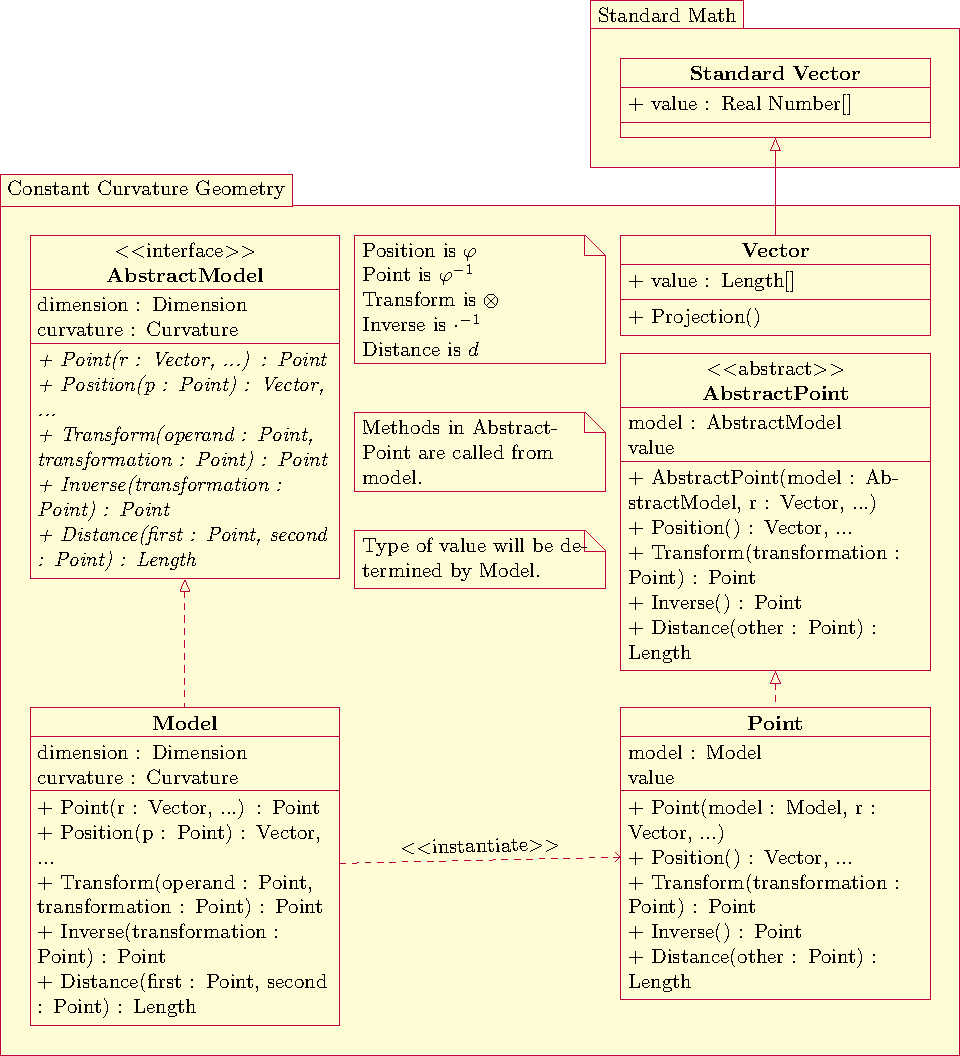
\includegraphics[width=\textwidth]{algorithm/modelclass.pdf}
    \caption{UML class diagram of the model}\label{ModelClassDiagram}
\end{figure}
\begin{figure}
    \centering
    % \import{figures/trigonometric}{2dplot}
    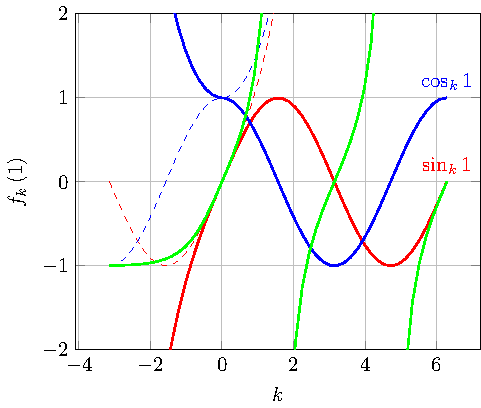
\includegraphics[width=\textwidth]{trigonometric/2dplot.pdf}
    \caption{Generalized trigonometric functions as function of $k$}\label{TrigonometryPlotted}
    \figurenote{This graph shows the value of generalized trigonometric functions as solid line and trigonometric and hyperbolic functions in the unused domain as dashed line.}
\end{figure}
\begin{figure}
    \centering
    % \import{figures/trigonometric}{sine}
    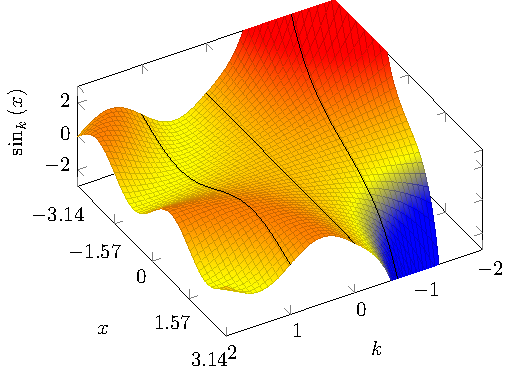
\includegraphics[width=\textwidth]{trigonometric/sine.pdf}
    \caption{Generalized sine function}\label{TrigonometrySinePlotted}
\end{figure}
\begin{figure}
    \centering
    % \import{figures/trigonometric}{cosine}
    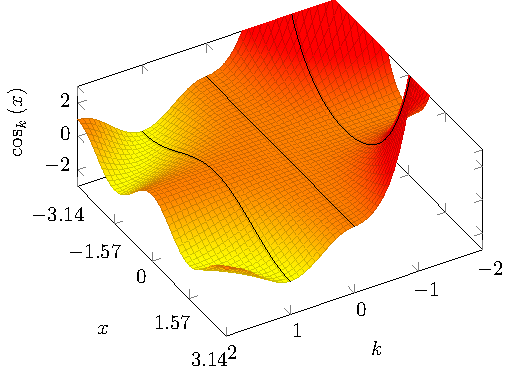
\includegraphics[width=\textwidth]{trigonometric/cosine.pdf}
    \caption{Generalized cosine function}\label{TrigonometryCosinePlotted}
\end{figure}
\begin{figure}
    \centering
    % \import{figures/trigonometric}{tangent}
    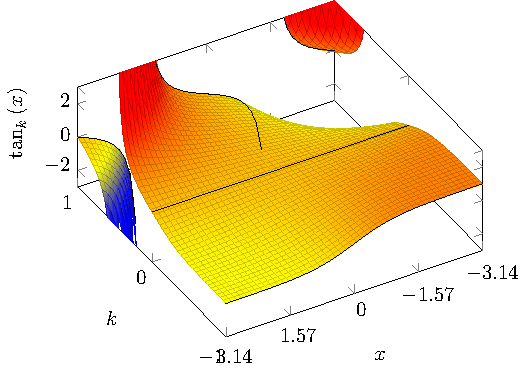
\includegraphics[width=\textwidth]{trigonometric/tangent.pdf}
    \caption{Generalized tangent function}\label{TrigonometryTangentPlotted}
\end{figure}
\end{document}